\subsection{Pix2Pix-Kernkonzepte}
\subsubsection{Generator}
Die Bildverarbeitung hat in den letzten Jahren durch den Einsatz tiefer neuronaler Netzwerke erhebliche Fortschritte gemacht. Im Mittelpunkt vieler dieser Fortschritte steht die U-Net-Architektur, die speziell für die Bildsegmentierung entwickelt wurde. Diese Architektur zeichnet sich durch ihre angeklügelte Kombination aus Encoder- und Decoder- Strukturen sowie durch den Einsatz von Skip-Verbindungen aus \cite{Isola}. 
 \newline
Bei der Encoder-Decoder-Struktur handelt es sich um einen Ansatz, bei dem das Eingangsbild zunächst durch den Encoder schrittweise reduziert wird. Dieser Prozess dient dazu, wesentliche Merkmale des Bildes zu erfassen. Anschließend wird das Bild durch den Decoder wiederhergestellt, indem die zuvor extrahierten Merkmale verwendet werden. Während dieser Prozesse besteht jedoch das Risiko des Informationsverlustes, insbesondere in den tieferen Schichten des Netzwerks.
Um dieses Problem zu adressieren, führt die U-Net-Architektur Skip-Verbindungen ein. Diese direkten Verbindungen zwischen korrespondierenden Schichten des Encoders und Decoders sorgen dafür, dass Detailinformationen nicht verloren gehen. Genauer gesagt, ermöglichen diese Verbindungen den direkten Informationsfluss zwischen jeweils äquivalenten Schichten, wodurch die Rekonstruktion des Bildes im Decoder mit einer höheren Genauigkeit erfolgt\cite{Isola}. \newline
Die Bedeutung von Skip-Verbindungen zeigt sich insbesondere in Anwendungen wie der Bild-zu-Bild-Übersetzung. Hier muss oft ein Bild mit niedriger Auflösung in ein Bild mit hoher Auflösung überführt werden, ohne dass Details verloren gehen. Die U-Net-Architektur, die angereichert mit diesen Verbindungen ist, ermöglicht daher eine feinere Rekonstruktion, die sowohl globale als auch lokale Informationen berücksichtigt \cite{Isola}.  \newline
Somit kann die U-Net-Architektur durch ihre Kombination aus Encoder-Decoder-Struktur und Skip-Verbindungen ein effektives Werkzeug für die Bildsegemtierung darstellen. Ihre Fähigkeit, sowohl globale Muster als auch feine Details zu berücksichtigen, macht sie zu einer bevorzugten Wahl für viele Bildverarbeitungsaufgaben \cite{Isola}. \newline
In Abbildung \ref{fig:unet} ist die typische U-Net-Architektur dargestellt. Die linke Seite des ''U'' repräsentiert den Encoder-Teil, der das Eingangsbild schrittweise reduziert und wesentliche Merkmale extrahiert. Die rechte Seite repräsentiert den Decoder-Teil, der das Bild mithilfe der extrahierten Merkmale rekonstruiert. Die horizontalen Linien repräsentieren die Skip-Verbindungen, die sicherstellen, dass Detailinformationen zwischen den korrespondierenden Schichten des Encoder und Decoders direkt übertragen werden \cite{Isola}. \newline 
In der Pix2Pix Technologie dient diese U-Net-Architektur als Generator. Er ist das zentrale Element, das für die Bild-zu-Bild-Übersetzung verantwortlich ist. Die Wahl der U-Net-Struktur für den Generator liegt in ihrer Fähigkeit, feinere Details und Kontextinformationen aus dem Eingangsbild beizubehalten, was für die Bild-zu-Bild-Übersetzung von entscheidender Bedeutung ist. Die Encoder-Decoder-Struktur des U-Net ermöglicht es dem Generator, den globalen Kontext des Bildes zu erfassen, während die Skip-Verbindungen sicherstelle, dass auch lokale Details im resultierenden Bild berücksichtigt werden \cite{Isola}.

\begin{figure}[h]
	\centering
	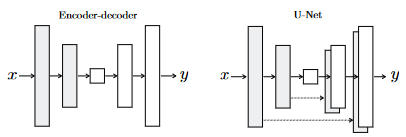
\includegraphics[width=0.7\linewidth]{./images/unet.png}
	\caption{Schematische Darstellung der U-Net-Architektur. Die Architektur besteht aus einem Encoder-Teil (links), einem Decoder-Teil (rechts) und Skip-Verbindungen zwischen korrespondierenden Schichten.}
	\label{fig:unet}
\end{figure}

\subsubsection{Diskriminator}

Im adversariellen Lernprozess spielen Generatoren und Diskriminatoren eine entscheidende Rolle. Während der Generator versucht, Daten zu erzeugen, die von echten Daten kaum zu unterscheiden sind, evaluiert der Diskriminator die vom Generator erzeugten Daten und versucht, zwischen echten und gefälschten Daten zu unterscheiden \cite{Isola}.\newline
Im Kontext von Generative Adverserial Networks (GANs), insbesondere im speziellen Fall des Pix2Pix GANs, spielt der PatchGAN-Diskriminator eine besonders wichtige Rolle. Der zentrale Unterschied dieses Diskriminators zu traditionellen Diskriminatoren liegt in der Art und Weise, wie er Bilder bewertet. Statt das gesamte Bild zu beurteilen, zerlegt der PatchGAN-Diskriminator das Bild in mehrere kleinere Bildabschnitte oder Patches und bewertet jeden Patch einzeln auf seine Echtheit \cite{Isola}. \newline
Ein solches Vorgehen hat den klaren Vorteil, dass feinere Strukturen und Details in den Bildern erkannt und beurteilt werden können. Durch diese segmentierte Beurteilung kann der Diskriminator besser einschätzen, ob die Struktur und Beschaffenheit eines bestimmten Bildteils realistisch ist. Dies ist besonders nützlich, da kleinere Unstimmigkeiten in den Bildern, die ein traditioneller Diskriminator möglicherweise übersieht, vom PatchGAN erfasst werden können. \newline
Ein weiterer Vorteil des PatchGAN-Diskriminators ist seine Skalierbarkeit. Da er auf festen Patchgrößen basiert, kann er flexibel auf Bilder unterschiedlicher Größen angewendet werden, ohne dass das zugrunde liegende Modell geändert werden muss. Dies führt nicht nur zu einer schnelleren Bildverarbeitung, sondern ermöglicht auch eine effiziente Ausführung auf großen Bildern. Darüber hinaus reduziert es potenzielle Kachelartefakte, die bei traditionellen Diskriminatoren auftreten können \cite{Isola}.\newline
Eine Metrik, die oft verwendet wird, um die Leistung des Diskriminator zu beurteilen, ist der FCN-Score. Dieser bewertet die Qualität der vom Generator erzeugten Bilder. Ein hoher FCN-Score zeigt, dass der Diskriminator erfolgreich echte von gefälschten Bildern unterscheiden kann. \newline
Der PatchGAN-Diskriminator kann wenn er effektiv eingesetzt wird, zu besseren und realistischeren Bildern im adverseriellen Lernprozess beitragen. Seine Fähigkeit, lokale Bildinformationen zu bewerten, ermöglicht es auch subtile Unterschiede in den Bildern zu erkennen, was zu einer verbesserten Qualität der generierten Bilder führt \cite{Isola}.

\subsubsection{L1-Verlustfunktion}

Die L1-Verlustfunktion, auch bekannt als Mean Absolute Error (MAE), spielt eine entscheidende Rolle im Pix2Pix-Modell, einem bedingten Generative Adversarial Network (cGAN) für Bild-zu-Bild-Übersetzungen. Diese Verlustfunktion misst den durchschnittlichen absoluten Unterschied zwischen den vorhergesagten und den tatsächlichen Werten, wodurch sie die Genauigkeit der generierten Bilder verbessert, insbesondere im Hinblick auf die niedrigen Frequenzen im Bild. Die L1-Verlustfunktion trägt somit maßgeblich zur Bewahrung der strukturellen Integrität und des Kontexts des Bildes bei \cite{Isola}. \newline
Die Verwendung des L1-Verlusts zusätzlich zum adversariellen Verlust im Pix2Pix-Modell ist von entscheidender Bedeutung. Während der adversarielle Verlust darauf abzielt, die generierten Bilder realistisch erscheinen zu lassen, konzentriert sich der L1-Verlust auf die Genauigkeit der niedrigen Frequenzen, um die strukturelle Integrität und den Kontext des Bildes zu bewahren. Diese Kombination ermöglicht es, sowohl die niedrigen als auch die hohen Frequenzen im Bild effektiv zu erfassen, was zu generierten Bildern führt, die sowohl strukturell korrekt als auch visuell ansprechend sind \cite{Isola}. \newline
Die L1-Verlustfunktion neigt jedoch dazu, bei den hohen Frequenzen unscharfe Ergebnisse zu liefern. Dies liegt daran, dass der L1-Verlust den Median der möglichen Werte bevorzugt, was zu einer Glättung der Bildtexturen führen kann. Um dieses Problem zu adressieren und scharfe, hochfrequente Details im Bild zu erhalten, wird der L1-Verlust im Pix2Pix-Modell mit einem adversariellen Verlust kombiniert. Diese synergetische Kombination von Verlustfunktionen ermöglicht es dem Pix2Pix-Modell, hochwertige Bild-zu-Bild-Übersetzungen durchzuführen, die sowohl visuell ansprechend als auch strukturell korrekt sind \cite{Isola}. \newline
Darüber hinaus hat sich die Kombination von L1-Verlust und adversariellen Verlust im Pix2Pix-Modell als nützlich für eine Vielzahl von Bild-zu-Bild-Übersetzungsproblemen erwiesen, einschließlich semantischer Segmentierung und Farbgebung. Durch die effektive Erfassung sowohl der niedrigen als auch der hohen Frequenzen im Bild trägt das Pix2Pix-Modell dazu bei, die Qualität der generierten Bilder zu verbessern und ihre Anwendbarkeit auf verschiedene Probleme zu erweitern \cite{Isola}.

\subsubsection{Training}

Der Trainingsprozess von Pix2Pix-Generative Adversarial Networks in der Bild-zu-Bild-Übersetzung geht über die bloße Erlernung der Abbildung von Eingabe- zu Ausgabebildern hinaus. Er umfasst auch das Entwickeln einer maßgeschneiderten Verlustfunktion, die speziell auf diese Art der Bildtransformation abgestimmt ist. Dieser umfassende Ansatz ermöglicht es Pix2Pix, sich flexibel an eine Vielzahl von Problemen anzupassen, die in der Vergangenheit unterschiedliche und spezialisierte Ansätze für die Verlustfunktion erforderten. Dadurch wird die breite Anwendbarkeit und Effektivität des Pix2Pix-Modells in verschiedenen Bildübersetzungsaufgaben deutlich. Pix2Pix benötigt eine spezifische Art von Trainingsdaten, um effektiv zu funktionieren. Die Trainingsdaten bestehen aus Paaren von Bildern, wobei jedes Paar ein Eingabebild und das entsprechende Ausgabebild enthält. Diese Bilder können 1-3 Kanäle aufweisen, was bedeutet, dass das Modell sowohl mit monochromatischen (Graustufen) als auch mit farbigen Bildern (RGB) arbeiten kann. Diese Flexibilität in der Kanalverarbeitung ermöglicht eine breitere Anwendung des Pix2Pix-Modells auf verschiedene Bildtypen. Die Bilder müssen nicht in einer bestimmten Weise vorverarbeitet werden, da das Modell direkt auf den Rohpixeln arbeitet. Diese Flexibilität in der Kanalverarbeitung und die Fähigkeit, direkt auf Rohpixeln zu arbeiten, unterstreichen die Vielseitigkeit des Pix2Pix-Modells. Dies wird weiter durch die sorgfältige Auswahl spezifischer Trainingsparameter und Hyperparameter-Optimierungsstrategien ergänzt. Der Adam-Grandientenoptimierungsalgorithmus ist eine Methode zur Optimierung des maschinellen Lernens, die auf adaptiven Schätzungen niedrigerer Ordnung basiert. Er passt automatisch die Lernrate während des Trainings an und eignet sich besonders gut für Probleme mit großen Datensätzen und/oder vielen Parametern. Durch empirische Tests hat sich herausgestellt das eine initiale Lernrate von 0.0002 und die Momentum-Parameter von $\beta1$ = 0.5 und $\beta$ = 0.999 optimal sind, um die Balance zwischen Lerngeschwindigkeit und Stabilität des Trainingsprozesses zu optimieren. Auch die Wahl einer kleinen Batchgröße, typischerweise 1, spielt eine entscheidende Rolle, um die Trainingseffizienz zu maximieren und qualitativ hochwertige Ergebnisse zu erzielen. Diese spezifischen Einstellungen der Trainingsparameter tragen maßgeblich dazu bei, das Potenzial des Pix2Pix-Modells voll auszuschöpfen.\cite{Isola}.\newline
Im Rahmen des Trainingsprozesses von Pix2Pix wird eine iterative Methode verwendet, bei der der Generator und der Diskriminator abwechselnd trainiert werden. Zunächst werden die Trainingsdaten vorbereitet, die aus Paaren von Eingabe- und Zielbildern besteht. Diese Bilder werden auf einen Wertebereich von -1 bis +1 skaliert. Diese Normalisierung ist wichtig, da sie zur Stabilisierung des Trainingsprozesses beiträgt. Sie ermöglicht es dem Modell, mit einem standardisierten Datensatz zu arbeiten, was die Lernrate und die Konvergenzgeschwindigkeit verbessert. Während des Tranings versucht der Generator, Bilder zu erzeugen, die vom Diskriminator nicht von realen Bildern unterschieden werden können. Der Diskriminator hingegen lernt, zwischen echten und vom Generator erzeugten Bildern zu unterscheiden. Eine Schlüsselkomponente dieses Prozesses ist die Verwendung einer zusammengesetzten Verlustfunktion, die sowohl den adverseriellen Verlust (bewertet vom Diskriminator) als auch den L1-Verlust(mittlerer absoluter Fehler zwischen generiertem Bild und Zielbild) umfasst. Dadurch wird der Generator dazu angehalten, realistische Übersetzungen der Eingabebilder zu generieren. Dieses Gleichgewicht zwischen Generator und Diskriminator ist entscheidend für die Effektivität des Pix2Pix-Modells \cite{Abdelmotaal2021}.
  

